\chapter{Transcendental Functions}

A \textbf{transcendental function} is a function that does not satisfy a polynomial equation whose coefficients are themselves polynomials, in contrast to an algebraic function, which does satisfy such an equation.

In other words, a transcendental function is a function that ``transcends'' algebra in the sense that it cannot be expressed in terms of a finite sequence of the algebraic operations of addition, multiplication, and root extraction.

Examples of transcendental functions include the \emph{exponential function}, the \emph{logarithm}, and the \emph{trigonometric functions}.
%\cite{wiki:transcendental}

Formally,

\begin{defn}
  An analytic function \(f(z)\) of the real or complex variables \(z_1, \ldots, z_n\) is \textbf{transcendental} if the \(n+1\) functions \(z_1, \ldots, z_n\) are algebraically independent.
  \cite{wiki:transcendental}
\end{defn}

\section{Natural Logarithms}
\begin{figure}[h]
  \begin{center}
    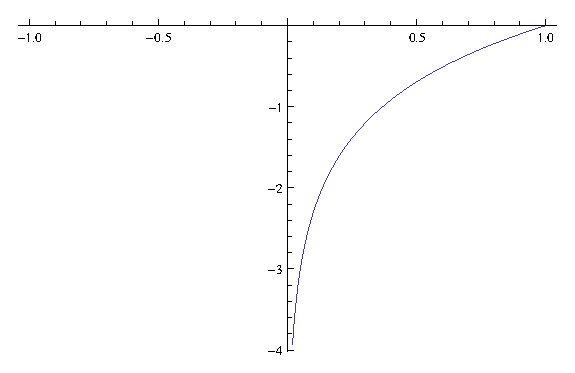
\includegraphics[width=0.4\textwidth]{continuous/transcend/natlog}
  \end{center}
  \caption{A plot of $f(x) =\ln x$.}
  \label{fig:natlog}
\end{figure}

\begin{defn}
  The \textbf{natural logarithm}\index{natural logarithm} is the function given by
  \begin{equation}
    \ln x = \int ^{x} _{1} \frac{1}{t} \ud t \text{,} \qquad x \in \mathbb{N}
  \end{equation}
\end{defn}
\begin{defn}
  The \textbf{number $e$} is that number in the domain of the natural logarithm satisfying
  \[ \ln{e}=1 \]
  It is roughly equal to
  \[2.7182818284590452353602874713526624977572470936999595\ldots\]
\end{defn}
\subsection{Algebraic Properties of the Natural Logarithm}

For any numbers $b>0$ and $x>0$, the natural logarithm satisfies the following rules:
\begin{table}[H]
    \begin{tabular}{p{3in}>\(p{3in}<\)}
      Product Rule      & \displaystyle{ \ln{bx}=\ln b + \ln x} \\\\
      Quotient Rule     & \displaystyle{ \ln{\frac{b}{x}}=\ln b - \ln x} \\ \\
      Reciprocal Rule   & \displaystyle{ \ln{\frac{1}{x}}=-\ln x} \\\\
      Power Rule        & \displaystyle{ \ln{x^r}=r \ln x \qquad \forall r \in \mathbb{R}}
    \end{tabular}
\end{table}
% \begin{equation}
% 	\ln{bx}=\ln b + \ln x
% \end{equation}
% \begin{equation}
% 	\ln{\frac{b}{x}}=\ln b - \ln x
% \end{equation}
% \begin{equation}
% 	\ln{\frac{1}{x}}=-\ln x
% \end{equation}
% \begin{equation}
% 	\forall r \in \mathbb{R} \quad \ln{x^r}=r \ln x
% \end{equation}
The number $e$ and its relationship to logarithms becomes especially important in integration,
where we manipulate its properties in calculus to solve equations and integrate functions we would not
otherwise be able to handle.

The inverse equations for $e^x$ and $\ln x$ are
\begin{equation}
  \forall (x>0)\big[e^{\ln x}=x\big]
  \label{eq:exinv1}
\end{equation}
\begin{equation}
  \forall x\big[\ln{(e^x)} =x\big]
  \label{eq:exinv2}
\end{equation}

The derivative of $e^x$ is very special, and it is
\begin{equation}
  \ddx e^x = e^x \ud x.
  \label{eq:ddxex}
\end{equation}


\section{Hyperbolic Functions}
Both \(\cos x\) and \(\sin x\) come from the formula for a circle.
\begin{equation}
  x^2 + y^2=r^2
  \label{eq:circle}
\end{equation}

But we can define other useful functions using the equation for a hyperbola.
\begin{equation}
  x^2-y^2=1
  \label{eq:hyperbola}
\end{equation}
Namely, \(\cosh x\) and \(\sinh x\).

In \ref{eq:hyperbola}, let \[ y \to \frac{e^x-e^{-x}}{2}\] to get \(\sinh x\).
Let \[ x \to \frac{e^x+e^{-x}}{2}\] to find \(\cosh x\).

We can prove that these still satisfy equation \ref{eq:hyperbola}:

\begin{proof}
  \begin{align*}
    1&=x^2-y^2 \\
    1&=\left( \frac{e^x+e^{-x}}{2} \right) - \left( \frac{e^x - e^{-x}}{2}
    \right)^2 \\
    1&=\frac{e^{2x}+2e^xe^{-x}+e^{-2x}}{4}-\frac{e^{2x}-2e^xe^{-x}+e^{-2x}}{4}
    \qedhere
  \end{align*}
\end{proof}
